\chapter{P3HT Validation}
\label{chap:p3ht_validation}

The following chapter contains unpublished work written by me with guidance from Dr. Jankowski.

\section{Summary}
 
A Jupyter notebook demonstrating the tools mentioned in this chapter can be found in \autoref{app:p3ht_nb}.

\section{Introduction}
The global climate crisis is the most pressing issue humanity faces today.
Consumption of fossil fuels for energy and transportation is the primary contributor to rising atmospheric $CO_{2}$ levels \citep{Solomon2009a}.
Changes in the climate influenced by atmospheric $CO_{2}$ are long-lasting, devastating, and inequitable, often impacting the poorest nations the hardest.
Global energy consumption is predicted to increase from 19 TW in 2020 to 27 TW in 2040 \citep{Mazzio2015, ieo2020}, so we must look to alternatives to power generation using fossil fuel.
Solar power represents one way to sustainably meet our energy demands, and the contribution of solar energy generation to the total green energy portfolio has opportunity to increase.
To persuade corporations to adopt solar power, however, it must be more profitable.
Despite improvements over the last 40 years, the cost of photovoltaic (PV) devices has prevented solar power from being a large part of the energy generation portfolio.
In order for solar power to be a viable option, large scale PV technology needs to be more economical and efficient \citep{Mazzio2015, Espinosa2012}.

Organic photovoltaics (OPVs) are a focus of this research because they represent the best opportunity for cost-effective solar power.
The theoretical efficiency limit (Shockley-Queisser limit) for a p-n single junction solar cell is about 30\% \citep{Shockley1961}.
Multijunction cells may achieve efficiencies that surpass this limit, but they often do not have lower energy payback times as their production is more costly.
\autoref{nrel} shows the efficiency gains made by single junction silicon and organic photovoltaic devices over the last 30 years.
These are merely a selection among the many categories of PV devices.
The trend of the silicon cells shows that the efficiency gain is leveling off as the devices approach the Shockley-Queisser limit.
OPV devices, however, still have a lot of room for improvement, and recent increases in efficiency reflect this.
\begin{figure}[h!]
    \centering
    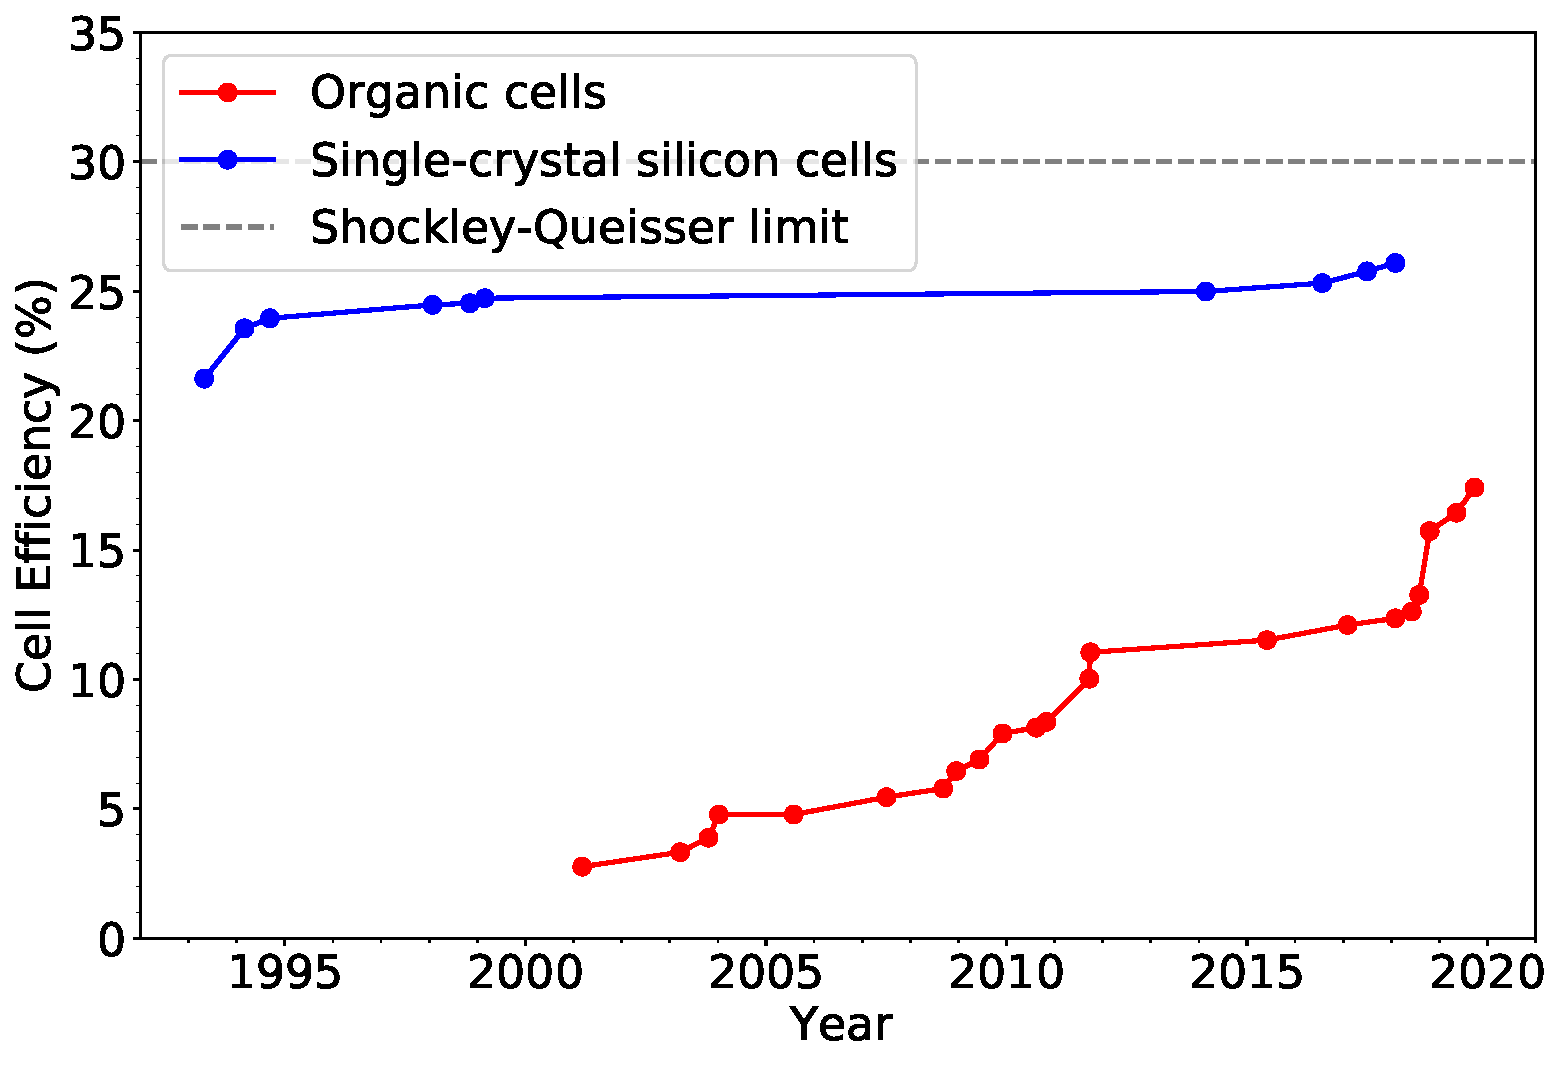
\includegraphics[width=0.8\linewidth]{figures/p3ht_val/NREL2020.pdf}
    \caption{Comparison of efficiencies in organic and silicon photovoltaic technologies from 1990 to present. The current state-of-the-art OPV, polymer-fullerene device coupled with a transition metal disulfide, achieves 17.4\% efficiency \citep{Lin2019}. Data taken from~\citet{NREL2020}.}\label{nrel}
\end{figure}
The potential of OPVs to achieve higher power conversion efficiencies depends on the morphology of the active layer. 
Molecular simulation can help to predict the combinations of donor and acceptor which will robustly self-assemble into a morphology best able to transport charge. 

A complication of the simulation of OPV polymers is that the properties which predict a device's efficiency, for example charge transport, span multiple length scales.
In order to model charge movement through a device, we need to know the position of individual atoms in order to discern the electronic environment and thus the likelihood of a charge hop, but we also need a bulk structure large enough that we can observe morphological features like the interdigitation of polymer lamellae to compare these morphologies to experiment.
But atomic resolution at length scales of hundreds of nanometers becomes computationally expensive, so simulating larger morphologies necessitates a simplified model.
By simplifying our model using coarse-graining techniques where multiple atoms are represented as a single bead we can more efficiently equilibrate larger length scales.

In additional to using a simplified model, the statepoint variables (including temperature, density, and solvent) must be carefully tuned to find the conditions under which the OPV morphology has the best self-assembly. 
A previous work from our lab, \citet{Miller2018}, performed a hundreds of molecular dynamics simulations of poly-3-hexylthiophene (P3HT) polymer across different temperatures and solvent quality in order to ascertain at which statepoints the morphology would self-assemble into the most ordered structure.
(Solvent quality, $\epsilon_{s}$, refers to a scaling factor on the non bonded forces.)
These hundreds of simulations were organized using custom python scripts which relied on creating and navigating a directory structure.
To quantify the degree of ordering, an order parameter was defined as being the ratio of thiophene moeities in "large" (n$\ge$6) clusters, where the clustering criteria takes into account the distance between thiophene centers and the angle between the planes of the thiophenes.
This analysis required selecting specific atoms from the trajectory file based on their index.
Simulated GIXS diffraction was used to compare the most highly ordered morphologies to experiment and they were found to show good agreement.
This work accomplished what it set out to do (validate a simplified model of P3HT) and was impressive in scope (hundreds of simulations!) and all the code is freely available to all, but how can we redesign these tools to be easier to use for the next molecule and the next user? 

%% transition here from Evan's work to mine
This work has a broad computational scope: managing a large parameter space, moving data between multiple different pieces of code, translating units, and performing analysis on selected particles from simulation trajectories.
Much of my work in the lab has been to design tools which makes these tasks more transparent, reproducible, usable, and extensible (TRUE) \citep{Thompson2020}.
If this project is going to have the desired impact (i.e., using molecular simulation to identify novel OPVs), every step of the process and the resulting data must be straightforward to reproduce and validate.
The nature of a multiscale simulation requires translation between formats and units and accurate handling of large data, and thus requires infrastructure to reduce error.
Although the molecular and computational scope of this project is broad, by using and building upon existing architectures and adhering to recent guidelines in the computational sciences community we can manage the multiscale nature of this project and contribute to reproducible science.
This chapter will demonstrate that we can reproduce and validate our P3HT morphologies while using MoSDeF tools to help our methods to be more TRUE.

\section{Statement of Need}
In order to sample the parameter space, we need to be able to spin up a large number of simulations (i.e., initializing our simulation volume, implementing the forcefield, and running the simulation) and accurately access each simulation output to perform analysis.
The analysis involves selecting the atoms that are part of a chemical moiety and calculating the distance and angle between each potential neighbor moiety. 
If the potential neighbor meets the clustering criteria, it is added to the cluster.
The order parameter can then be calculated as the ratio of the number of the moieties in large clusters vs the total number.

Before we address issues in the implementation, it is important to note how we solved issues related to installing the software stack.
Often this step goes unmentioned, but installation of software packages and managing dependencies can be a huge hurdle for computational scientists. 
To prevent this, we have built pipelines for all our code repositories (using GitHub Actions) which automatically build docker containers from each tagged version of the repository and the latest master branch. 
This allows our software to be used without ever having to manually install it or manage its dependencies. 
Not only does this make our software stack easier to use, but it makes it more portable---we can have the exact same environment on our school cluster or XSEDE. 
And if someone wants to reproduce our work, they can access the exact container we used.

% transition

Although the application of the united-atom model to our P3HT system was not overly complicated as it only contained 3 types, it required manual atom typing, which presented another hurdle to applying this method to a new and perhaps more complicated compound. 
By using the foyer forcefield dissemination and atom-type engine \cite{foyer} our atom types can be automatically assigned based on the chemical connectivity. This allows us to more easily extend to new compounds.

Calculating the order parameter originally depended on a workflow that was hard-coded for P3HT and selected specific atom indices---this depended on the particle order in the simulation being the same every time, which it was because routine initialization methods were used, but it did not allow for the method to be applied to other compounds.

%% method then tools or tools then method?
\section{Tools}

Next we will discuss the various tools used in this project. \autoref{fig:p3ht-workflow} gives an overview of how these tools work together to perform the structural analysis.
\begin{figure}[h!]
    \centering
    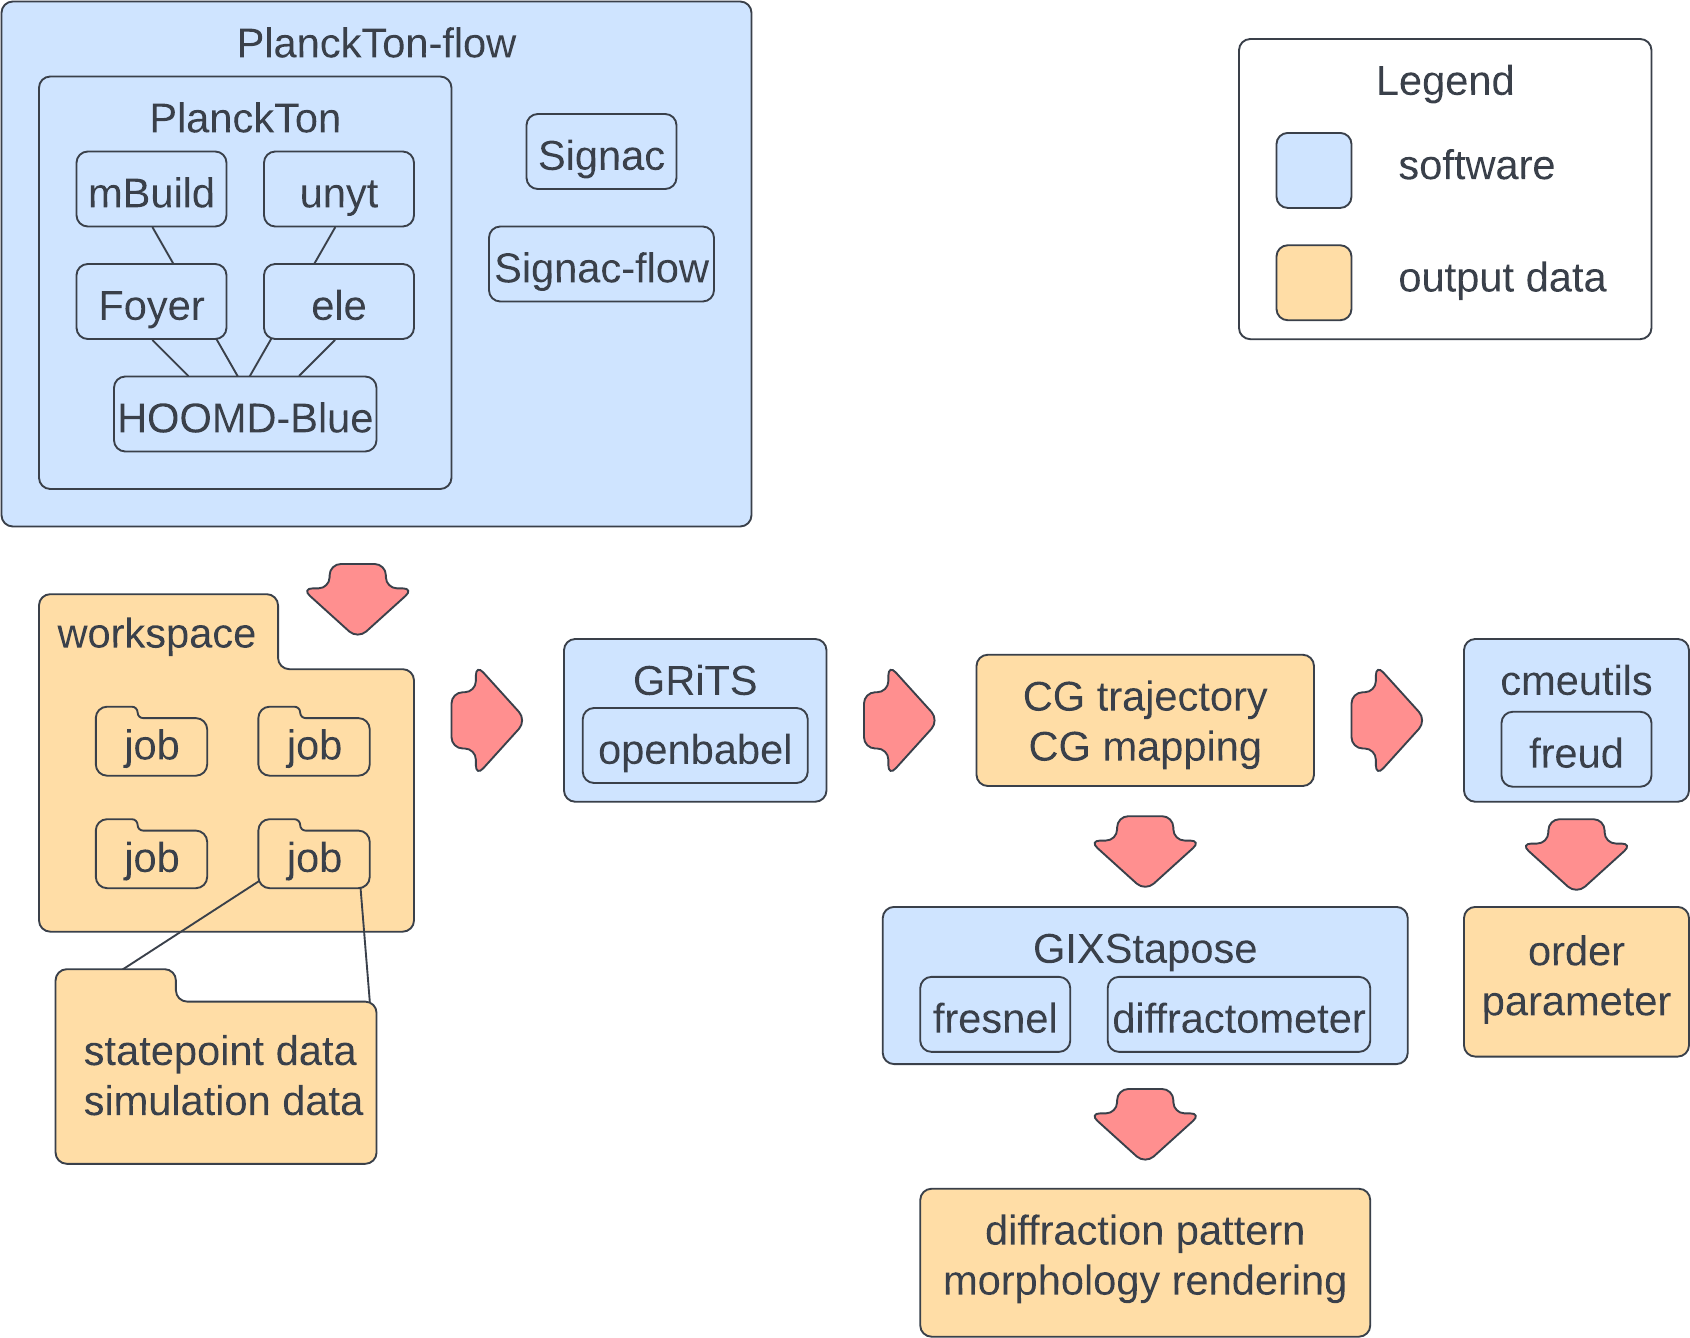
\includegraphics[width=0.8\linewidth]{figures/p3ht_val/workflow.png}
    \caption{Overview of the structural analysis workflow. First, the workspace is created in the PlanckTon-flow framework and all simulations are run. Then GRiTS is used on the output simulation data to find the thiophene centers. Finally, the order parameter function in cmeutils is used to calculate the order parameter of each simulation trajectory and GIXStapose is used to perform GIXS analysis.}\label{fig:p3ht-workflow}
\end{figure}

\subsection{PlanckTon}
In order to initialize simulations in a reproducible way, we have designed PlanckTon: a wrapper for the initialization, management, and submission of organic photovoltaic molecular dynamics simulations \citep{planckton, Jankowski2019}.
This project was started by my lab mates Mike, Evan, and Matty.
The PlanckTon software includes some OPV compounds commonly used in our lab to guarantee that all simulations are initialized with the exact same starting compound; however, the workflow is designed to easily accept any MoSDeF compatible chemical input file format including SMILES strings. 
The code base also ships with custom XMLs for OPLS-UA and GAFF and a separately packaged GAFF XML \citep{DeFever}, but is compatible with any Foyer XML. 
The initialization procedure of PlanckTon is as follows: First the user selects a compound or mixture of compounds, the number of said compounds, the temperature, the density, and the solvent parameter. 
In order to more robustly achieve high density morphologies, the simulation volume is initialized at a lower density and then shrunk down to the desired density at high temperature\cite{Jankowski2013,Marsh2014,Jones2017,Henry2017a,Miller2018}. 
The creation of our simulation volume, the forcefield atom-type assignment, and the creation of the HOOMD force objects is completely handled by mBuild and foyer in the MoSDeF framework\citep{mbuild,foyer}.
By using the modular, general system initialization of the mBuild and foyer, we get two benefits: (1) we draw on the knowledge base of the MoSDeF community--more users means we can find and resolve errors more quickly, and (2) we can more easily incorporate the system initialization in our other projects. 
Once the system and forces are initialized, PlanckTon uses the NVT ensemble via the Nosé-Hoover thermostat \citep{Martyna1994d, Martyna1996} as implemented in the HOOMD-Blue molecular dynamics engine \citep{hoomd}. 
The initial velocities and angular momenta are randomly assigned from the Maxwell-Boltzmann distribution.
By having our entire process scripted, we can have everything about our process documented and available for scrutiny and reduce the potential human error inherent when switching between codes or transferring files.
Through PlanckTon-flow, this tool is supported by the Signac framework, which handles the parameter space initialization and management and submission to various computing clusters. Because this workspace is created using signac, signac can be used to navigate it. This allows to reference our data via the statepoint (e.g., what temperature and $\epsilon_{s}$ it was run at) without ever having to create or manage a complicated directory structure or naming scheme.

Planckton is unique, but there exist other tools to manage molecular dynamics simulations. There is a web-based application that facilitates MD simulation using cloud computing services and automates related tasks \citep{Nicolas-Barreales2021} and a command line tool that automates many common MD tasks \citep{Rackers2018}, but I have not seen a pure python implementation which can also manage a large dataspace.

Recent updates to Planckton have allowed it to be more TRUE: 
Updating to HOOMD 2 allowed us to use the HOOMD simulation initialization functions in mBuild. This allows the package to be more modular and useable by others; any improvements or bugfixes needed in the \lstinline{create_hoomd_simulation} function can be contributed back to mBuild, which allows the whole community to benefit.
We have added automated docker container builds.
Planckton's initialization procedure has been generalized to allow starting compounds to be loaded from SMILES strings or any input file and these untyped compounds can be typed on the fly using any foyer compatible forcefield.
Planckton now supports other neighborlists, which allows better sampling of sparse systems. 
Planckton also allows for user specified temperature ramps, allowing users to perform temperature annealing, a technique used in OPV active layer synthesis.
In order to be more clear about the units used in PlanckTon, the unyt package is used to handle all unit conversions. This package allows for values to be tagged with their unit and then all conversions can be handled by the package.

\subsection{GRiTS}
GRiTS was developed as a tool to assist in applying a coarse-grain mapping and to backmap a coarse-grain system to a fine one. 
Although the fine-graining capabilities are in the early stages and still under development, the coarse-graining is robust enough to apply a mapping to an entire system trajectory. 
This mapping can also be used to pick out specific chemical moieties from a morphology. 
GRiTS works using SMARTS matching---implemented in OpenBabel---to map atomic indexes to coarse grain beads. 
Once all the atomic indices are assigned to a bead, then bonds are inferred between coarse-grain beads based on the atomistic bonding scheme. 
For example, if an atom in bead A is bonded to an atom in bead B, beads A and B are assumed to be bonded. 
When looking at an entire simulation trajectory, the SMARTS matching algorithm can be prohibitively expensive.
So GRiTS uses the following simplifying assumptions: Chemical bonds are not formed or broken over the course of the simulation---this allows only the first frame of the trajectory to be used for mapping. 
Using only the first frame of the trajectory is also useful because this way the molecules in the system can be guaranteed to be chemically reasonable---i.e., the bonds and angles are not distorted, aromatic systems should be planar, etc. 
It is also assumed that if molecules have the same number of atoms, they have the same chemical structure. 
This allows us to use the clustering algorithms of implemented in the Freud analysis library to break the snapshot into molecules and only perform SMARTS matching on each molecule type, then extrapolate the mapping out to other molecules of the same type.

When working with a UA system, GRiTS can also infer hydrogen positions and bonding. This allows for SMARTS strings to find matches in UA systems. The hydrogen inferring method uses OpenBabel and requires that the first frame of the trajectory be chemically reasonable.

There are other tools which handle creating coarse-grain mappings such as VOTCA \citep{Ruhle2009}. 
This tool will crate a coarse grain trajectory from an atomistic one given an XML file mapping which requires the user to specify everything from the atom types involved in the bead to the bond and angle information.
VOTCA also has many other functions that GRiTS does not such as coarse-graining (including potential development), charge-transport, and excitation transport.
But it can be said that creating a mapping with GRiTS may be more intuitive.

\subsection{GIXStapose}
GIXStapose is a package which allows users to connect the real space view of a chemical structure to its simulated grazing incidence X-ray scattering (GIXS) pattern. (The name ``GIXStapose'' is a portmanteau of ``GIXS'' and ``juxtapose.'') GIXStapose works by translating the structure information in many chemical input files into the format need by the diffractometer package and the fresnel ray tracing library \cite{Diffract, Jones2017, fresnel}. The package has an interactive graphical user interface (GUI), but is completely modular and can be run in a scripted fashion to generate reproducible figures and diffraction patterns along with translation of units. This work was presented at Scipy2020 \cite{gixstapose-scipy}. 

\section{Methods}
\subsection{Generate simulation data}
A planckton-flow workspace of 40 simulations sweeping over temperature and solvent parameter ($\epsilon_{s}$) was initialized with 100 united-atom (UA) P3HT 16-mers parameterized with GAFF. (The compound can be found in planckton as "P3HT-16-gaff" and the forcefield is "gaff-custom".) All the nonbonded forces used a cutoff value of 8.91 \AA (2.5 times the largest sigma value). The target density for all was 0.56 $\frac{g}{cm^{3}}$. All simulations used a timestep of 2 fs and started by shrinking the box from 125 times the the target volume to the target volume (789 nm$^3$) at 629 K, with a thermostat coupling value (tau) of 2 ps, run over 0.2 ns. Once the shrink step was finished, each simulation was run at its own combination of temperature and $\epsilon_{s}$ ranging from 125, 188 to 629 K and 0.2 to 1.0, respectively. These runs used a thermostat coupling value (tau) of 0.6 ps and were run for 200 ns. All were run in the cmelab/planckton\_gpu:v0.6.1 docker container. 

%% equilibration analysis?

The GRiTS \lstinline{CG_System} class was used to find indices of atoms in thiophenes using SMARTS string ``c1cscc1'' and inferred hydrogens. This created a new coarse-grain trajectory file with beads at thiophene centers and a json file which contains the SMARTS string which generates the mapping and the atom indices in the atomistic trajectory as a key value pair.

The \lstinline{order_parameter} function in cmeutils was designed to use the coarse grain trajectory and the mapping to calculate the average order parameter of the last ten frames of the trajectory. An angle cutoff 10 $^{\circ}$ and a distance cutoff of 6 \AA was used as the clustering criteria.

\begin{figure}
    \centering
    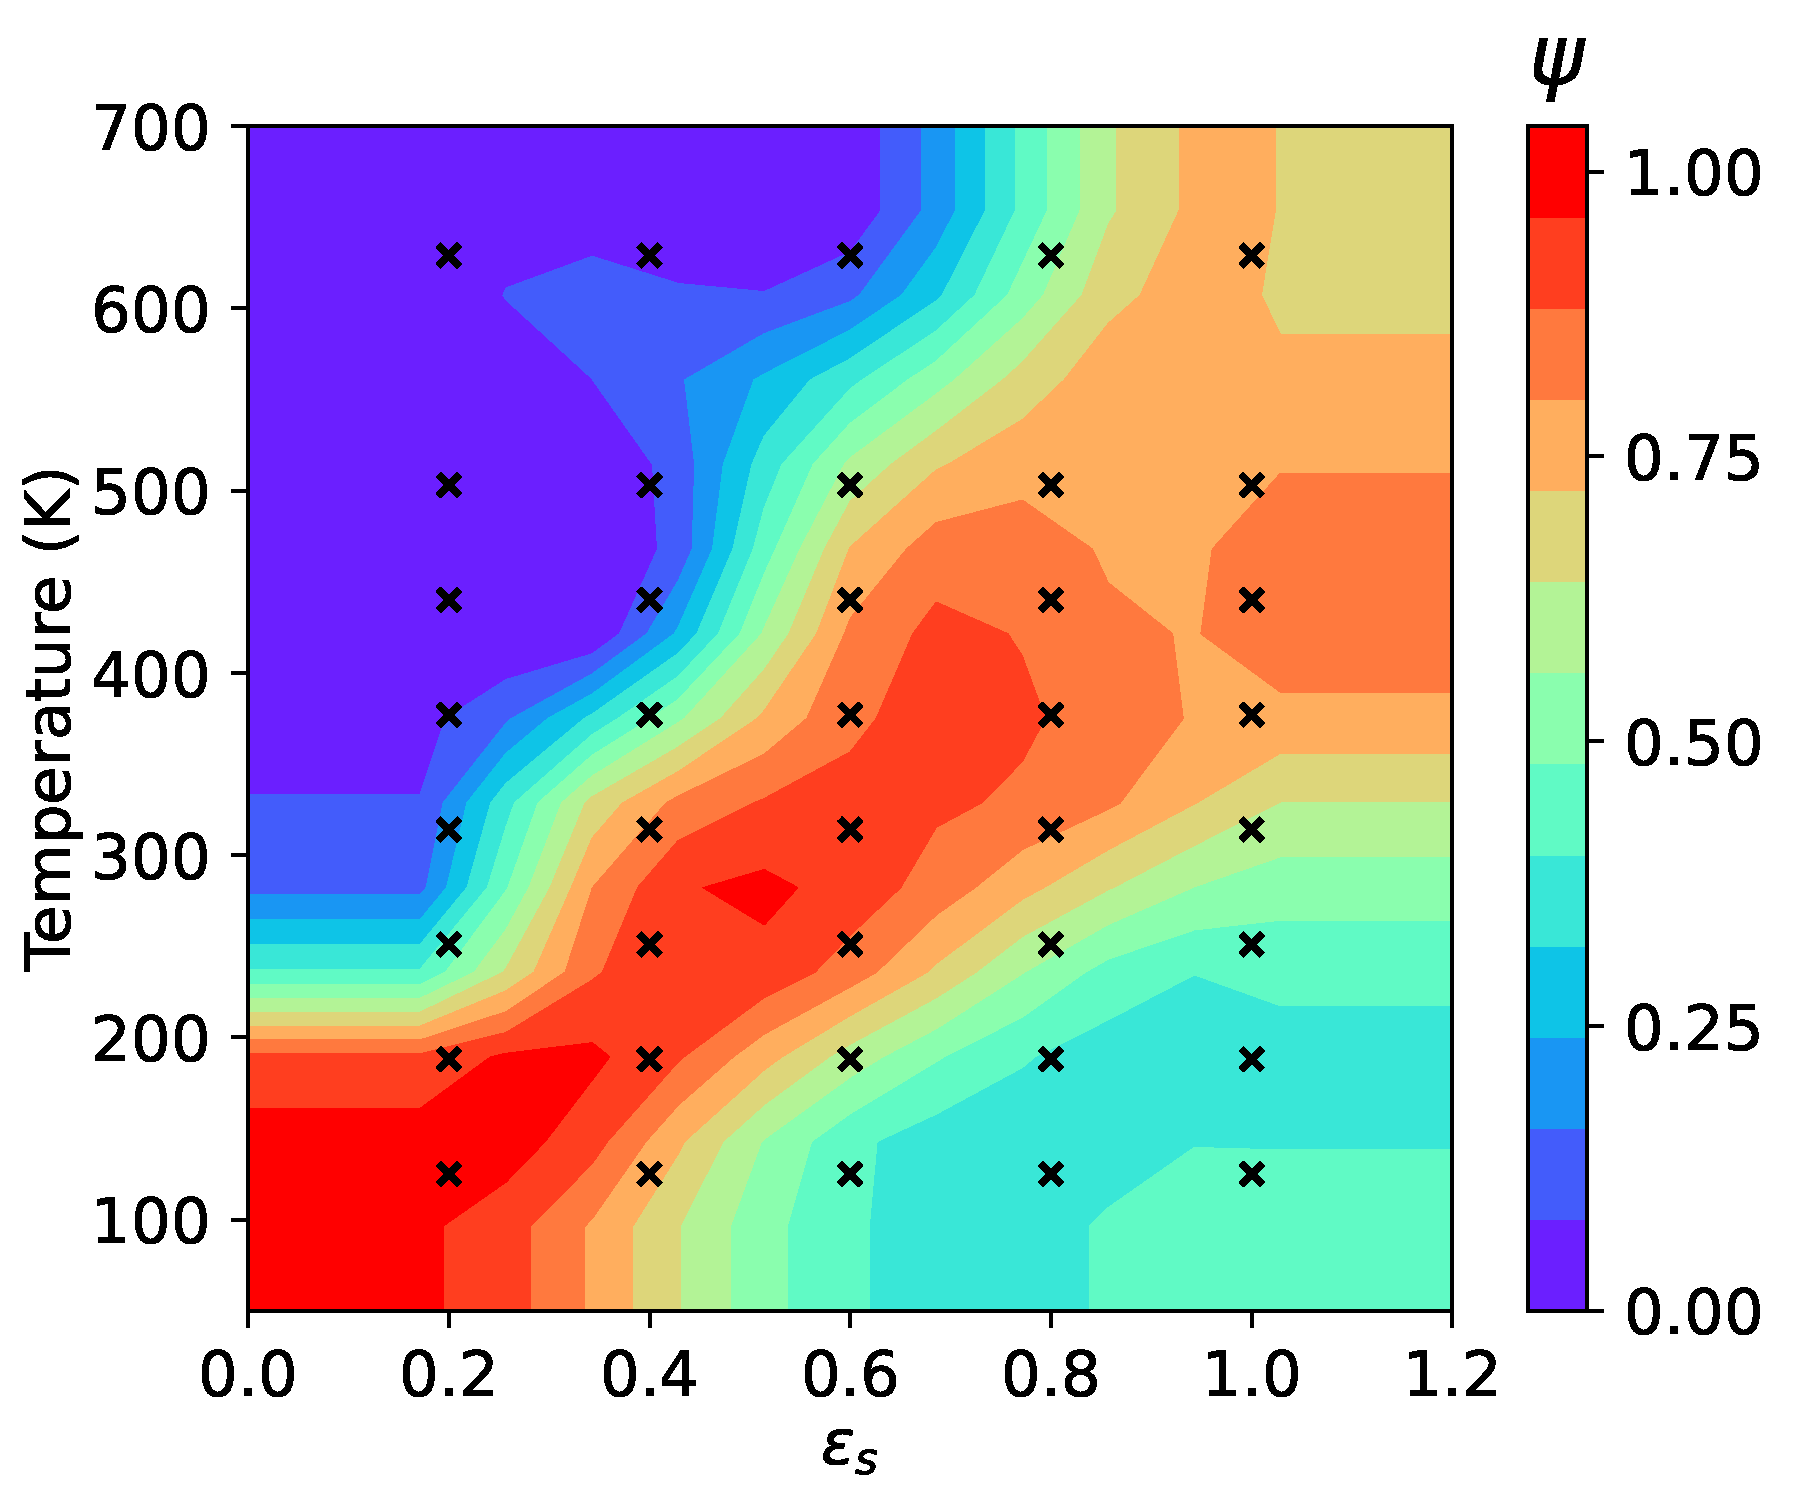
\includegraphics[width=0.8\linewidth]{figures/p3ht_val/order_parameter.pdf}
    \caption{Degree of ordering, $\psi$, of P3HT. Red regions denote high order, blue regions are disordered. Each black "x" indicates a measurement, values between are interpolated.}\label{order} %% im copying evan's caption for now--change later
\end{figure}

\autoref{order} was created using that order parameter data and scipy interpolate RectBivariateSpline adjusting the final z values such that no order parameter was greater than 1 or less than 0.
%% I will provide notebook, environment.yml for analysis, and zipped planckton-flow workspace
%%  \citep{Fothergill2022} zenodo dataset (planckton-flow workspace)

Next the high order regions were further examined using GIXS analysis (see \autoref{highorder-dp}).

can show correlation between high order parameter and peaks in GIXS vs low order and no peaks in GIXS (see \autoref{loworder-dp}).

%% This camera information and how it was chosen is given in the notebook
%%Camera
%%   position = [8.133, 5.203, 43.865],
%%   look_at =  [0.000, 0.000, 0.000],
%%   up =       [0.900, 0.424, -0.101],
%%   height =   31.896
\begin{figure}
    \centering
    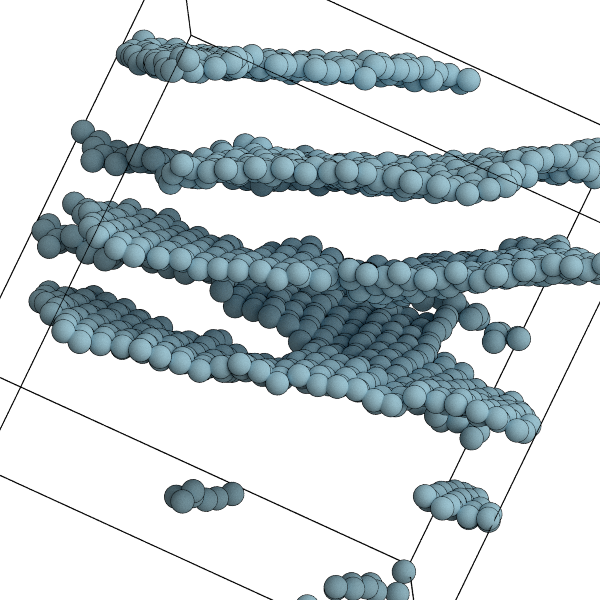
\includegraphics[width=0.8\linewidth]{figures/p3ht_val/cg-trajectory_scene.png}
    \caption{Thiophene centers for $\epsilon_{s}$: 0.4, T: 251K.}\label{highorder-centers}
\end{figure}

\begin{figure}
    \centering
    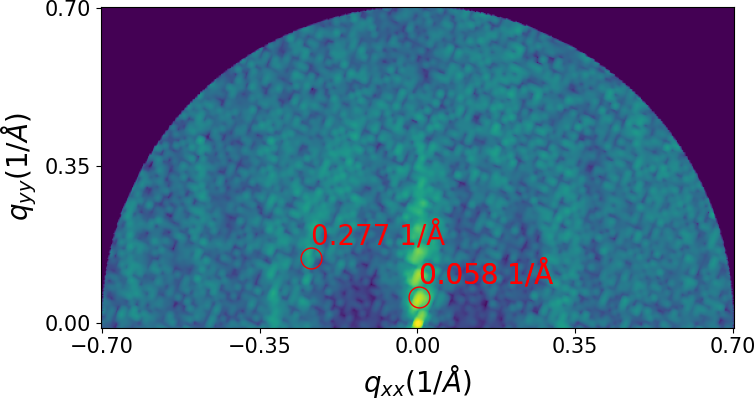
\includegraphics[width=0.8\linewidth]{figures/p3ht_val/cg-trajectory_dp0.png}
    \caption{Diffraction pattern for thiophene centers for $\epsilon_{s}$: 0.4, T: 251K.}\label{highorder-dp}
\end{figure}

These peaks correspond to distances of 17.24 \AA, 3.61 \AA; \citet{Duong2013} report a lamellar spacing of 16.5 \AA~ and a pi-stacking spacing of 3.83 \AA~ for neat P3HT.

\begin{figure}
    \centering
    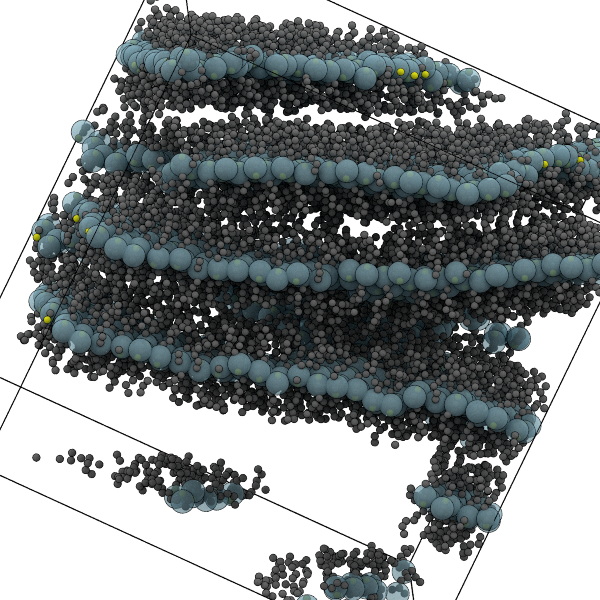
\includegraphics[width=0.8\linewidth]{figures/p3ht_val/cg-overlay_scene.png}
    \caption{Overlay of thiophene bead centers (translucent blue) with united atom carbon (grey) and sulfur (yellow) in p3ht trajectory for $\epsilon_{s}$: 0.4, T: 251K. }\label{centers-overlay}
\end{figure}


\begin{figure}
    \centering
    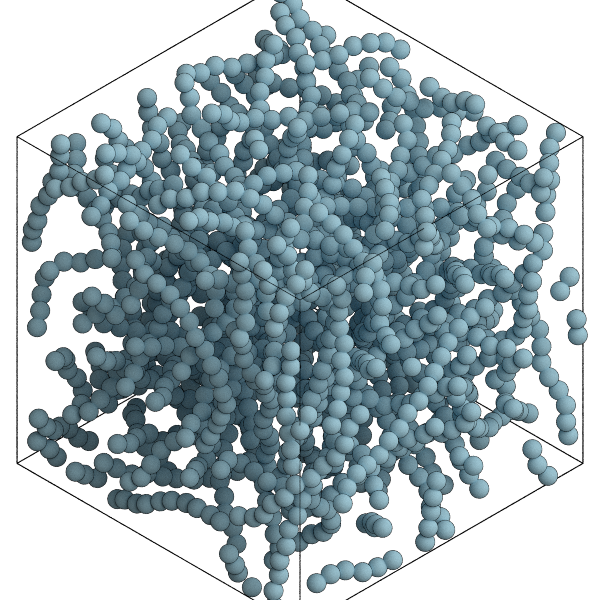
\includegraphics[width=0.8\linewidth]{figures/p3ht_val/cg-trajectory-amorphous_scene.png}
    \caption{Thiophene centers for $\epsilon_{s}$: 0.2, T: 629K.}\label{loworder-centers}
\end{figure}

\begin{figure}
    \centering
    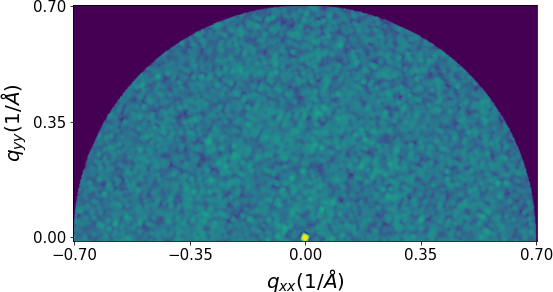
\includegraphics[width=0.8\linewidth]{figures/p3ht_val/cg-trajectory-amorphous_dp0.png}
    \caption{Diffraction pattern for thiophene centers for $\epsilon_{s}$: 0.2, T: 629K.}\label{loworder-dp}
\end{figure}


\section{Results and Discussion}

New students were able to use PlanckTon to use XSEDE hours?
Comparisons of Order parameter plot
Comparisons of order parameters themselves
Order parameter range in test suite?

How have we made this work more TRUE?
By using mBuild with foyer in PlanckTon to initialize our simulations, we can easily use different input file formats including smiles strings and any foyer forcefield. 
Using GRiTS to select the desired part of the molecule removes any need for manual indexing. This allows us to more easily extend the order parameter calculation to other planar, conjugated molecules like perylene or ITIC.
By using the Signac framework we can quickly and easily sample the necessary parameter space without needing to manually create or manage directories. 
We've also implemented semantic versioning in planckton with version tagged docker containers which helps users to get the same code state.
PEP8 compliant code and docstrings are ensured by using the pre-commit git hook manager to automatically lint the code with black, isort, pydocstyle.
Along with jupyter notebook examples, GRiTS also has a sphinx readthedocs page.
By building on existing code, we work with a community of open-source molecular simulators. 

Hopefully this software ecosystem will continue to be dynamic and evolving. Future changes to planckton will hopefully involve updating to HOOMD version 3, which is at the time of writing still in beta. The work of \citet{Miller2018a} has shown the importance of polydisperse polymer lengths and their ability to form tie-chains for charge transport simulations. 
Tools for initializing disperse polymers are under development and would be a great addition to planckton \cite{polybinder}.

% tie it back to the intro